%!TEX root = Report.tex
\chapter{Laboratory Description}\label{sec:experimentalsetup}

\section{Experimental Setup}
The experiment consists of a tank filled with warm water at $T_i=51 ^\circ C$ and a test section connected to it as shown schematic in Figure \ref{pic:schematic}. The water from the reservoir is constantly pumped through the test section so that all components should roughly be heated up to $T_i$. 
\begin{figure}[H]
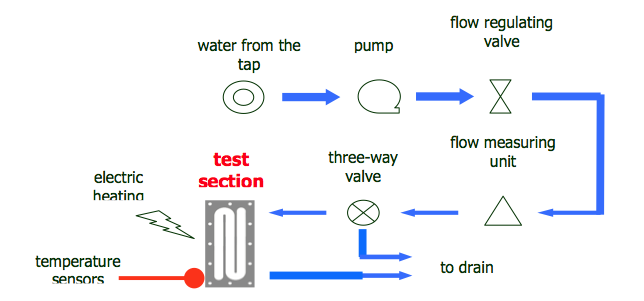
\includegraphics[width=1.0\textwidth]{pics/schematic}
\caption{Schematic Setup of the Experiment}
\label{pic:schematic}
\end{figure}
The test section itself contains an aluminum back plate with a TLC-sheet on its surface. In the cooling channel some v-shaped obstacles are arranged to cause a turbulent flow. The front plate is made out of plexiglas allowing the camera to capture pictures of the TLC-sheet.
\begin{figure}[H]
\mbox{
\subfigure[]{
\includegraphics[width=.25\textwidth]{pics/testsection1}
\label{pic:testsection1}}\quad
\subfigure[]{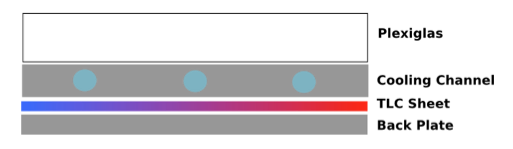
\includegraphics[width=.7\textwidth]{pics/testsection2}
\label{pic:testsection2}}}
\caption{Testsection (a) with obstacles (b) schematic}
\label{pic:testsection}
\end{figure}

\section{Experimental Procedure}
As mentioned above water is pumped through the closed loop for about an hour to obtain the uniform  temperature $T_i= 51 ^\circ C$ in all components. Measurements start as soon as the three-way valve is opened (t=0) and a cold water pulse runs through the test section at $T_\infty=10 ^\circ C$. A CCD camera linked to a computer captures the change of color of the liquid crystals foil caused by the temperature drop. A simultaneously started MATLAB file saves the camera's 100 pictures and post processes the data.
